\documentstyle[12pt,psfig,draft,lscape,array]{nature-ejb}

\textwidth16cm\textheight24.8cm\voffset-2.3cm\hoffset+1.5cm
\voffset-1cm

\def\simlt{\mathrel{\hbox{\rlap{\hbox{\lower4pt\hbox{$\sim$}}}\hbox{$<$}}}}
\def\simgt{\mathrel{\hbox{\rlap{\hbox{\lower4pt\hbox{$\sim$}}}\hbox{$>$}}}}

\def\ale{\mathrel{\hbox{\rlap{\hbox{\lower4pt\hbox{$\sim$}}}\hbox{$<$}}}}
\def\age{\mathrel{\hbox{\rlap{\hbox{\lower4pt\hbox{$\sim$}}}\hbox{$>$}}}}

\def\nodata{---}

\def\ra#1#2#3{#1$^{\rm h}$#2$^{\rm m}$#3$^{\rm s}$}
\def\dec#1#2#3{$#1^\circ#2'#3''$}

\newcommand{\hst}{\textit{HST}}
\newcommand{\swift}{\textit{Swift}}
\newcommand{\ergcms}{erg cm$^{-2}$ s$^{-1}$}
\newcommand{\uJy}{\mbox{$\mu$Jy}}
\newcommand{\Tburst}{\mbox{$T_{\rm GRB}$}}

\def\spose#1{\hbox to 0pt{#1\hss}}

\begin{document}

\title{\large \bf The Birth of a Relativistic Outflow in the Unusual
$\gamma$-ray Transient Swift\,J164449.3+573451}

\author{
B.~A.~Zauderer\affiliation[1]
     {Harvard-Smithsonian Center for Astrophysics, 60 Garden St., 
      Cambridge, MA 02138, USA},
E.~Berger\affiliationmark[1],
A.~M.~Soderberg\affiliationmark[1],
A.~Loeb\affiliationmark[1],
R.~Narayan\affiliationmark[1],
D.~A.~Frail\affiliation[2]
     {National Radio Astronomy Observatory, P.O. Box 0, Socorro, 
      NM 87801, USA},
G.~R.~Petitpas\affiliationmark[1],
A.~Brunthaler\affiliation[3]
     {Max-Planck-Institut f$\ddot{u}$r Radioastronomie, Auf dem 
      H$\ddot{u}$gel 69, 53121 Bonn, Germany},
R.~Chornock\affiliationmark[1],
J.~M.~Carpenter\affiliation[4]
     {Department of Astronomy, California Institute of Technology, 
      Pasadena, CA 91125, USA},
G.~G.~Pooley\affiliation[5]
     {Mullard Radio Observatory, Cavendish Laboratory, Cambridge 
      UK},
K.~Mooley\affiliationmark[4],
S.~R.~Kulkarni\affiliationmark[4],
R.~Margutti\affiliation[6]
     {INAF Osservatorio Astronomico di Brera, via Bianchi 46, 
      Merate 23807, Italy},
D.~B.~Fox\affiliation[7]
     {Department of Astronomy, Pennsylvania State University, 
      University Park, PA 16802, USA},
E.~Nakar\affiliation[8]
     {School of Physics \& Astronomy, Tel Aviv University, Tel 
      Aviv 69978, Israel},
N.~A.~Patel\affiliationmark[1],
N.~H.~Volgenau\affiliation[9]
     {California Institute of Technology, Owens Valley Radio 
      Observatory, Big Pine, CA 93513, USA},
T.~L.~Culverhouse\affiliationmark[9],
M.~F.~Bietenholz\affiliation[10]
     {Hartebeesthoek Radio Astronomy Observatory, PO Box 443,
      Krugersdorp, 1740 South Africa}$^,$\affiliation[11]
     {Department of Physics and Astronomy, York University, 
      Toronto, Ontario, Canada},
M.~P.~Rupen\affiliationmark[2],
W.~Max-Moerbeck\affiliationmark[4],
A.~C.~S.~Readhead\affiliationmark[4],
J.~Richards\affiliationmark[4],
M.~Shepherd\affiliationmark[4],
S.~Storm\affiliation[12]
     {Department of Astronomy, University of Maryland, College 
      Park, MD 20742},~\&
C.~L.~H.~Hull\affiliation[13]
     {Radio Astronomy Laboratory, University of California, Berkeley, 
      CA 94720}
}

\date{\today}{}
\headertitle{Birth of a Relativistic Outflow in
Swift\,J164449.3+573451}
\mainauthor{Zauderer et al.}

\summary{Active galactic nuclei (AGN), powered by long-term accretion
onto central supermassive black holes, produce\cite{bbr84}
relativistic jets with lifetimes of $\simgt 10^6$ yr that preclude
observations at birth.  Transient accretion onto a supermassive black
hole, for example through the tidal disruption\cite{hil75,ree88} of a
stray star, may therefore offer a unique opportunity to observe and
study the birth of a relativistic jet.  On 2011 March 25, the {\it
Swift} $\gamma$-ray satellite discovered\cite{burrows11} an unusual
transient source (Swift\,J164449.3+573451) potentially
representing\cite{bgm+11,ltc+11} such an event.  Here we present the
discovery of a luminous radio transient associated with
Swift\,J164449.3+573451, and an extensive set of observations spanning
centimeter to millimeter wavelengths and covering the first month of
evolution.  These observations lead to a positional
coincidence\cite{gcn11854} with the nucleus of an inactive galaxy, and
provide direct evidence for a newly-formed relativistic outflow,
launched by transient accretion onto a $10^6$ M$_\odot$ black hole.
While a relativistic outflow was not predicted in this scenario, we
show that the tidal disruption of a star naturally explains the
high-energy properties, radio luminosity, and the inferred rate of
such events.  The weaker beaming in the radio compared to
$\gamma$-rays/X-rays, suggests that radio searches may uncover similar
events out to redshifts of $z\sim 6$.}
\maketitle

\noindent{\it This paper has been submitted to Nature. You are free to 
use the results here for the purpose of your research.  In accordance 
with the editorial policy of Nature, we request that you not discuss 
this result in the press.  If you have any question or need 
clarifications please contact Ashley Zauderer (bzauderer@cfa.harvard.edu) 
or Edo Berger (eberger@cfa.harvard.edu).}

Upon the discovery\cite{burrows11} of Swift\,J164449.3+573451, and the
identification of a galaxy at a redshift\cite{ltc+11} of $z=0.354$
within the {\it Swift} X-ray localization region ($1.4''$ radius), we
initiated radio observations of the transient on 2011 March 29.36 UT
with the Expanded Very Large Array (EVLA) at a frequency of 5.8 GHz
and discovered an unresolved source with a flux density of 
$310\pm 7$~$\mu$Jy.  Astrometric matching demonstrated that the radio 
source coincides with the galaxy nucleus (Figure~\ref{fig:image}),
subsequently confirmed\cite{ltc+11} with other data.  A follow-up EVLA
observation 0.9~d later revealed that the source brightened to $530\pm
10$~$\mu$Jy, thereby conclusively linking the X-ray/$\gamma$-ray
transient and the galaxy for the first time.  The galaxy exhibits no
evidence\cite{ltc+11} for an active nucleus (see Figure 1 in online
Supplementary Information; SI), and the lack of previous 
$\gamma$-ray/X-ray activity argues\cite{burrows11} against an
AGN flare origin.

We carried out additional observations at multiple frequencies
spanning $1-345$ GHz with several cm- and mm-wave facilities 
(see SI Table 1). The spectral energy distribution (SED) in this 
frequency range on 2011~March~30~UT ($\Delta t\approx 5$~d) is well 
described by a power law with $F_\nu\propto\nu^{1.3\pm 0.1}$ up to 
$F_\nu(345\,{\rm GHz})=35\pm 1$~mJy.  The steep power law requires 
self-absorbed synchrotron emission.  The weak near-infrared (NIR) 
variability\cite{ltc+11} indicates $F_\nu(2.5\,{\rm\mu m})\approx 
0.1$~mJy, while the lack of optical variability leads\cite{ltc+11} 
to an upper bound of $F_\nu(0.64\,{\rm \mu m})\simlt 2$ $\mu$Jy.  
The SED therefore peaks in the millimeter band, with a best-fit 
rest-frame peak frequency and flux density of $\nu_p\approx 6\times 
10^{11}$~Hz and $F_{\nu,p} \approx 80$~mJy, respectively (
Figure~\ref{fig:sed}).  The non-detection of optical variability 
requires significant rest-frame extinction of $A_V\simgt 3$ mag, 
further supporting a nuclear origin. Subsequent SEDs at 
$\Delta t\approx 10$, $15$, and $22$~d exhibit
significant evolution, with $\nu_p\propto t^{-1.3}$ and
$F_{\nu,p}\propto t^{-0.8}$ (Figure~\ref{fig:sed}).

For synchrotron sources there is a well-defined minimum energy,
achieved\cite{rea94} near equipartition between the fractional
energies in the relativistic electrons ($\epsilon_e$) and magnetic
fields ($\epsilon_B$).  This condition defines\cite{che98} the
equipartition radius: $\theta_{\rm eq}= 110\,d_{\rm
L,Mpc}^{-1/19}\,F_{\rm\nu, p,mJy}^{9/19}\,\nu_{\rm p,GHz}^{-1}$
$\mu$as.  From the March~30~UT SED we find $\theta_{\rm eq}\approx 1$
$\mu$as ($r_{\rm eq}\approx 1.5\times 10^{16}$ cm) and hence mildly
relativistic expansion with a Lorentz factor of $\Gamma\approx 2$.  A
more detailed model that accounts\cite{kn09} for relativistic effects
leads to a similar result, $r_{\rm eq}\approx 1\times 10^{16}$ cm and
$\Gamma\approx 1.2$ (see SI).  From the observed SED temporal
evolution we find that the source continues to expand relativistically
with nearly constant velocity (see SI text).  Extrapolating the linear
trend in radius we find a formation epoch in the range 2011 March
23-26 UT, in excellent agreement with the initial $\gamma$-ray
detection on 2011 March 25 UT (see SI Figure 2).  This provides 
independent evidence for a newly-formed relativistic outflow.

An angular size of a few $\mu$as will inevitably lead to variability
in the low frequency radio emission due to interstellar scintillation,
with the amplitude of modulation depending\cite{gn06} on the ratio of
the source size ($\theta_s$) to the Fresnel scale ($\theta_F$).  For
the line of sight to Swift\,J164449.3+573451 the maximum modulation
($m_p\approx 1$) is expected\cite{cl02} at $\nu_0\approx 10$~GHz, for
$\theta_s\approx\theta_F\approx 1$~$\mu$as.  The observed modulation
inferred from our detailed radio light curves is tens of percent at
$5-7$ GHz and a few percent at $15$~GHz (Figure~\ref{fig:lc}), leading
to a projected radius of $\theta_s\approx 5$ $\mu$as, or $\Gamma
\approx 5$.  This provides independent evidence for a relativistic
outflow.  Our radio observations with Very Long Baseline
Interferometry (VLBI) at a frequency of 22 GHz place an upper bound on
the size of $r\simlt 0.8$ pc, consistent with the synchrotron and
scintillation analyses, and providing an upper bound on the lifetime
of the event of $\simlt 1.7$ yr for an expansion with $\Gamma\approx
2$ (see SI text).

The mean X-ray luminosity during the four radio epochs exceeds the
synchrotron peak by a factor of $\sim 10^3$ and therefore requires a
distinct origin (Figure~\ref{fig:sed}).  One potential mechanism to
generate the large X-ray luminosity is inverse Compton (IC) scattering
of radio synchrotron photons by the relativistic electrons
(synchrotron self-Compton: SSC), but from the relativistic model we
find a predicted SSC X-ray luminosity of only $\approx 2\times
10^{45}$ erg s$^{-1}$ (see SI).  Similarly, although order of
magnitude variations in brightness are seen in the X-rays, our
detailed radio light curves do not reveal coincident variations as
would be expected for SSC (Figure~\ref{fig:lc}).  We therefore
conclude that the X-ray emission is dominated by a distinct, and more
compact emission region, most likely at the base of the outflow.

Having established the birth of a relativistic outflow, coincident
with the nucleus of the host galaxy, we briefly describe a model to
power the outflow through transient accretion\cite{bgm+11} onto a
supermassive black hole (SMBH).  The host galaxy luminosity,
$M_B\approx -18.2$ mag, implies\cite{gh07} a modest SMBH mass of $\sim
10^5-10^6$ M$_\odot$.  The duration of the bright early phase in the
X-ray light curve, $\sim 10^5$ s, coincides with the debris fallback
time for a solar-mass star tidally disrupted at a pericenter distance
$R_p\sim 13 (M_{\rm SMBH}/10^6\,{\rm M}_\odot)^{-5/6}$ Schwarzschild
radii.  The most bound stellar debris is expected to feed the black
hole at an initial rate of\cite{sq09} $\sim (\frac{1}{2}{\rm
M_\odot})/10^5$.  With a radiative efficiency of $\simgt 1\%$ at $\sim
R_p$, this can account for the observed X-ray luminosity.  However,
this luminosity is $\sim 10^3$ times the Eddington limit for a $\sim
10^6$ M$_\odot$ black hole, leading inevitably to a highly collimated
outflow, the origin of the radio-emitting relativistic outflow found
here.

We conclude with several key implications of our results.  First, our
initial estimate of the energy, $E_K\approx 3\times 10^{50}$ erg at
$\Delta t\approx 22$ d (see SI Table 2), corresponds to the Eddington
luminosity of a $10^6$ M$_\odot$ black hole, lending support to the
tidal disruption scenario, and suggesting that the X-ray/$\gamma$-ray
emission is collimated by a factor of $\sim 10^3$.  Long-term radio
monitoring will test this result by providing precise
beaming-independent calorimetry\cite{fwk00,sb11} of the true energy
release.  Continued radio observations will also uniquely probe the
density structure near a previously-dormant supermassive black hole as
the ambient medium is swept up by the relativistic outflow.  
From the existing data we find $n_e$~$\propto$~r$^{-2.4}$ (see SI).
Second,
with continued expansion we expect that VLBA observations will resolve
the radio source on a timescale of $\sim 2$~yr, and directly confirm
the relativistic expansion; from the observed flux density evolution
we predict a peak of a few mJy at several GHz on this timescale,
within the reach of the VLBA.  Third, from the detection of a single
such event in 6 years of {\it Swift} operations we infer a rate of
$\sim 0.1$ Gpc$^{-3}$ yr$^{-1}$, much lower than the
predicted\cite{wm04} tidal disruption rate of $\sim 10^2-10^3$
Gpc$^{-3}$ yr$^{-1}$, or upper limits from current radio
surveys\cite{bow11} of $\simlt 10^3$ Gpc$^{-3}$ yr$^{-1}$.  This
suggests that the properties of Swift\,J164449.3+573451 are
exceedingly rare; if due to jet collimation, the implied beaming
fraction is $\sim 10^{3}$, consistent with the ratio of the observed
X-ray luminosity to the Eddington limit and the radio-inferred energy.
Finally, past searches\cite{kb99,gbm+08,cbk+11} for tidal disruption
events have focused on the expected\cite{sq09} bright optical/UV and
soft X-ray emission, but the large optical extinction and associated
soft X-ray absorption in Swift\,J164449.3+573451 suggest that radio
observations may provide a cleaner signature.  This is particularly
true if the X-ray/$\gamma$-ray emission is beamed by a factor of $\sim
10^3$.  With the EVLA and the Atacama Large Millimeter Array, similar
events are detectable to $z\sim 6$.

\clearpage
\begin{thebibliography}{10}
\bibitem[{Begelman}, {Blandford} \& {Rees}<1>]{bbr84} {Begelman},
M.~C., {Blandford}, R.~D.  \& {Rees}, M.~J. {Theory of extragalactic
radio sources}.  \newblock {\it Reviews of Modern Physics} {\bf 56},
255--351 (1984).

\bibitem[{Hills}<2>]{hil75} {Hills}, J.~G. {Possible power source of
Seyfert galaxies and QSOs}.  \newblock {\it Nature} {\bf 254}, 295--298
(1975).

\bibitem[{Rees}<3>]{ree88} {Rees}, M.~J. {Tidal disruption of stars by
black holes of 10 to the 6th-10 to the 8th solar masses in nearby
galaxies}.  \newblock {\it Nature} {\bf 333}, 523--528 (1988).

\bibitem[{Burrows} {\it et~al.}<4>]{burrows11} {Burrows}, D.~N. {\it
et al.} {Discovery of the Onset of Rapid Accretion by a Dormant
Massive Black Hole}.  \newblock {\it Submitted to Nature}.

\bibitem[{Bloom} {\it et~al.}<5>]{bgm+11} {Bloom}, J.~S., {Giannios},
D., {Metzger}, B.~D., {Cenko}, S.~B., {Perley}, D.~A. {\it et al.} {A
relativistic jetted outburst from a massive black hole fed by a
tidally disrupted star}.  \newblock {\it ArXiv:1104.3257}, (2011).

\bibitem[{Levan} {\it et~al.}<6>]{ltc+11} {Levan}, A.~J., {Tanvir},
N.~R., {Cenko}, S.~B., {Perley}, D.~A., {Wiersema}, K. {\it et al.}
{An extremely luminous panchromatic outburst from the nucleus of a
distant galaxy}.  \newblock {\it ArXiv:1104.3356}, (2011).

\bibitem[{Berger} {\it et~al.}<7>]{gcn11854} {Berger}, E., {Levan},
A., {Tanvir}, N.~R., {Zauderer}, A., {Soderberg}, A.~M.  {\it et al.}
{GRB 110328A / Swift J164449.3+573451: Radio-optical/NIR astrometry.}
\newblock {\it GRB Coordinates Network, Circular Service} {\bf 1854},
1 (2011).

\bibitem[{Readhead}<8>]{rea94} {Readhead}, A.~C.~S. {Equipartition
brightness temperature and the inverse Compton catastrophe}.
\newblock {\it Astrophys. J.} {\bf 426}, 51--59 (1994).

\bibitem[{Chevalier}<9>]{che98} {Chevalier}, R.~A. {Synchrotron
Self-Absorption in Radio Supernovae}.  \newblock {\it Astrophys.~J.}
{\bf 499}, 810--819 (1998).

\bibitem[{Kumar} \& {Narayan}<10>]{kn09} {Kumar}, P. \& {Narayan},
R. {GRB 080319B: evidence for relativistic turbulence, not internal
shocks}.  \newblock {\it Mon.~Not.~R.~Astr.~Soc.} {\bf 395}, 472--489
(2009).

\bibitem[{Goodman} \& {Narayan}<11>]{gn06} {Goodman}, J. \& {Narayan},
R. {Fitting Formula for Flux Scintillation of Compact Radio Sources}.
\newblock {\it Astrophys.~J.} {\bf 636}, 510--527 (2006).

\bibitem[{Cordes} \& {Lazio}<12>]{cl02} {Cordes}, J.~M. \& {Lazio},
T.~J.~W. {NE2001.I. A New Model for the Galactic Distribution of Free
Electrons and its Fluctuations}.  \newblock {\it ArXiv:0207156},
(2002).

\bibitem[{Greene} \& {Ho}<13>]{gh07} {Greene}, J.~E. \& {Ho}, L.~C. {A
New Sample of Low-Mass Black Holes in Active Galaxies}.  \newblock
{\it Astrophys.~J.} {\bf 670}, 92--104 (2007).

\bibitem[{Strubbe} \& {Quataert}<14>]{sq09} {Strubbe}, L.~E. \&
{Quataert}, E. {Optical flares from the tidal disruption of stars by
massive black holes}.  \newblock {\it Mon.~Not.~R.~Astr.~Soc.} {\bf
400}, 2070--2084 (2009).

\bibitem[{Frail}, {Waxman} \& {Kulkarni}<15>]{fwk00} {Frail}, D.~A.,
{Waxman}, E.  \& {Kulkarni}, S.~R. {A 450 Day Light Curve of the Radio
Afterglow of GRB 970508: Fireball Calorimetry}.  \newblock {\it
Astrophys.~J.}  {\bf 537}, 191--204 (2000).

\bibitem[{Shivvers} \& {Berger}<16>]{sb11} {Shivvers}, I. \& {Berger},
E. {A Beaming-Independent Estimate of the Energy Distribution of Long
Gamma-Ray Bursts: Initial Results and Future Prospects}.  \newblock
{\it Astrophys. J. in press}, 2011.

\bibitem[{Wang} \& {Merritt}<17>]{wm04} {Wang}, J. \& {Merritt},
D. {Revised Rates of Stellar Disruption in Galactic Nuclei}.
\newblock {\it Astrophys.~J.} {\bf 600}, 149--161 (2004).

\bibitem[{Bower}<18>]{bow11} {Bower}, G.~C. {Constraining the Rate of
Relativistic Jets from Tidal Disruptions Using Radio Surveys}.
\newblock {\it Astrophys.~J.} {\bf 732}, L12--L15 (2011).

\bibitem[{Komossa} \& {Bade}<19>]{kb99} {Komossa}, S. \& {Bade},
N. {The giant X-ray outbursts in NGC 5905 and IC 3599:() hfill
Follow-up observations and outburst scenarios}.  \newblock {\it
Astr.~Astrophys.}  {\bf 343}, 775--787 (1999).

\bibitem[{Gezari} {\it et~al.}<20>]{gbm+08} {Gezari}, S., {Basa}, S.,
{Martin}, D.~C., {Bazin}, G., {Forster}, K. {\it et al.} {UV/Optical
Detections of Candidate Tidal Disruption Events by GALEX and CFHTLS}.
\newblock {\it Astrophys.~J.} {\bf 676}, 944--969 (2008).

\bibitem[{Cenko} {\it et~al.}<21>]{cbk+11} {Cenko}, S.~B., {Bloom},
J.~S., {Kulkarni}, S.~R., {Strubbe}, L.~E., {Miller}, A.~A. {\it et
al.} {PTF10iya: A short-lived, luminous flare from the nuclear region
of a star-forming galaxy}.  \newblock {\it ArXiv:1103.0779}, (2011).

\end{thebibliography}

%\hspace{2in}

\clearpage
%\noindent$\bf{Supplementary~ Information}$ is linked to the online version of the
%paper at www.nature.com/nature.

%\hspace{1in}

\noindent$\bf{Acknowledgements}$  E.B.~is supported in part by funds 
from NASA.  A.~L.~is supported in part by NSF and NASA grants.  
R.M.~acknowledges support from a Swift ASI grant and from the Ministry 
of University and Research of Italy.  E.N.~is partially supported by IRG 
and ISF grants.  The EVLA and VLBA are operated by the NRAO, a facility
of the NSF operated under cooperative agreement by AUI.  The SMA is
a joint project between the SAO and the ASIAA, and is funded by the 
Smithsonian Institution and the Academia Sinica.  CARMA development and 
operations are supported by the NSF under a cooperative 
agreement, and by the Associates of the California Institute of Technology, 
the University of Chicago, and the states of California, Illinois, and Maryland.
The AMI arrays are supported by the University of Cambridge and the STFC.  
This work is partially based on observations with the 100-m telescope of 
the MPIfR at Effelsberg.  This work made use of data supplied by the UK 
Swift Science Data Centre at the University of Leicester.

\hspace{1in}

\noindent$\bf{Author~Contributions}$  A.Z. and E.B. designed and 
coordinated the radio observations and 
analysis among all instruments reported here.  A.Z. and D.A.F. 
performed EVLA observations, data reduction and analysis.  
G.R.P. observed the source with the SMA, and along with N.A.P. 
reduced and analyzed the SMA observations.  CARMA observations 
were set up, reduced and analyzed by A.Z., J.M.C. and S.R.K.  
S.S. and C.L.H.H. obtained the first CARMA observations.  
N.H.V. and T.L.C. facilitated quick response CARMA observations.  
R.C. implemented and analyzed MMT and Gemini optical observations.  
K.M. performed observations with the OVRO 40-m and analyzed results, 
with advice from S.R.K., A.C.S.R., J.R., M.S., and W.M.  G.G.P. 
performed observations with the AMI Large Array and analyzed the 
results.  A.M.S., A.B., M.F.B. and M.P.R. planned observations 
with the VLBA and Effelsberg.  A.B. reduced the VLBI data.  
R.M. analyzed and modeled the X-ray data.  A.L., R.N. and E.N. 
provided the theoretical model for a tidal disruption event.  
The paper was synthesized by A.Z. and E.B. with the primary text 
written by E.B. and portions of the SI written by E.B., A.Z., R.C., 
K.M. and A.B.  D.B.F. provided feedback on the manuscript.   
All authors discussed the results and commented on the manuscript.

\hspace{1in}

\noindent$\bf{Author~Information}$  Correspondence and requests for materials
should be addressed to A.Z. (bzauderer@cfa.harvard.edu) or
E.B. (eberger@cfa.harvard.edu).


\clearpage
\begin{figure}
\centerline{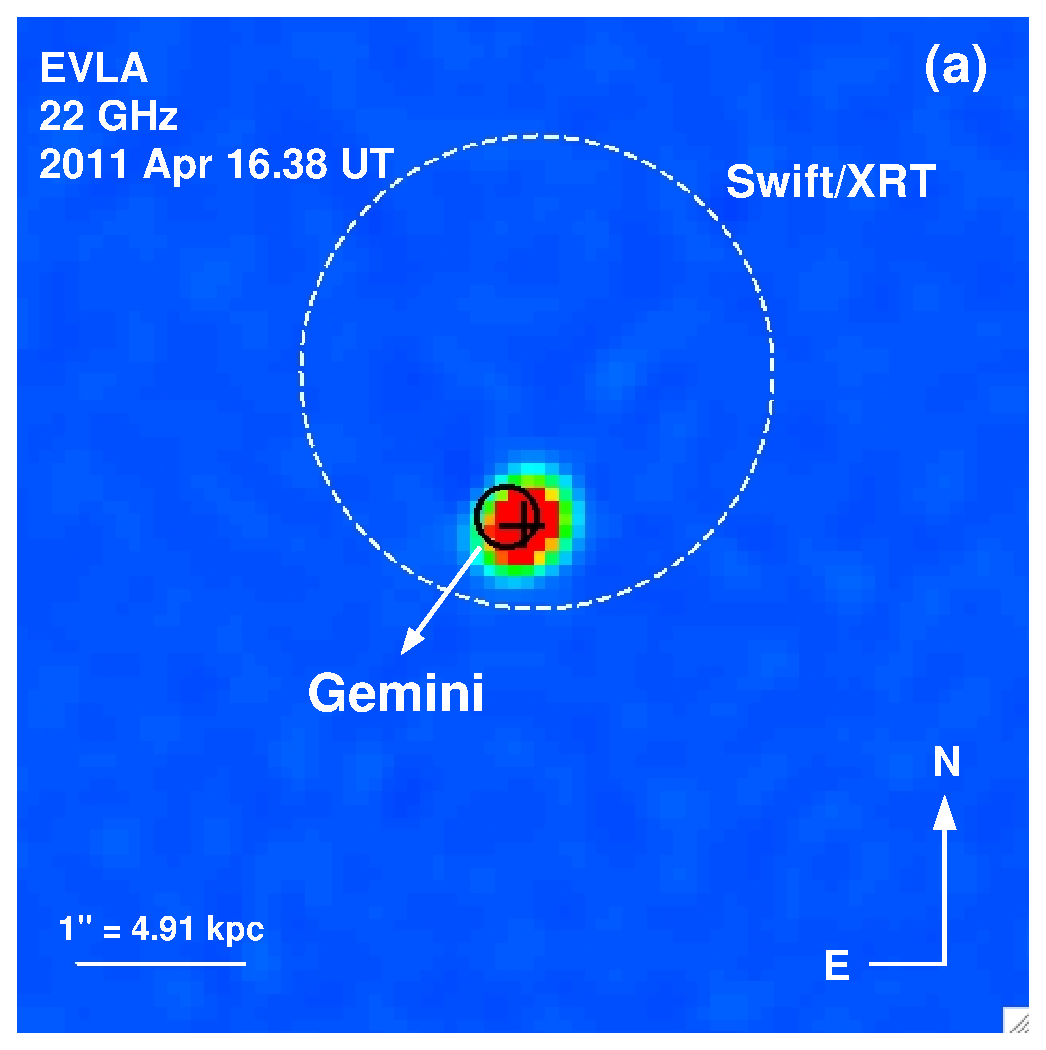
\psfig{file=figure1a.eps,width=2.9in,angle=0}\hfill 
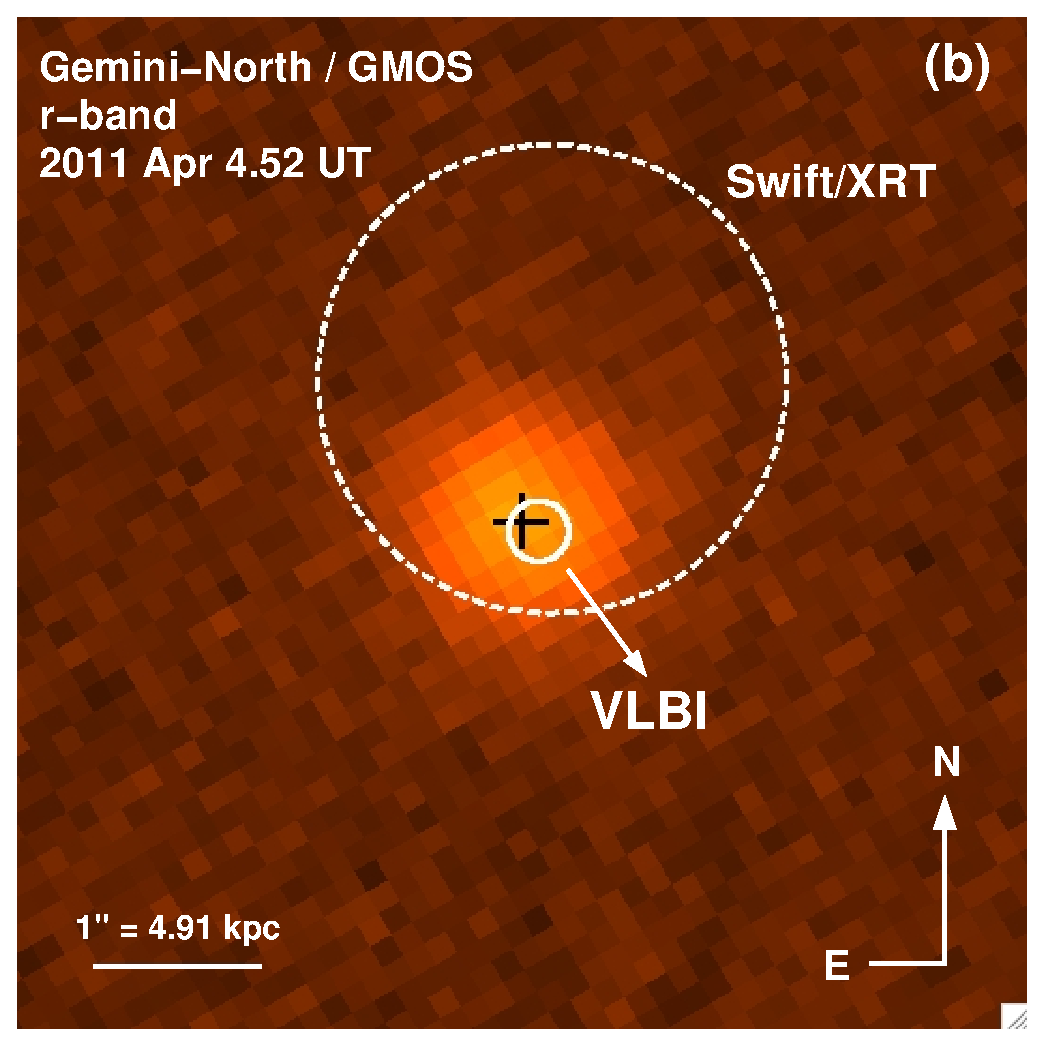
\psfig{file=figure1b.eps,width=2.9in,angle=0}}
\caption[]{\small 
Radio and optical images of Swift\,J164449.3+573451
and its host galaxy reveal a positional alignment between the
transient and the center of the galaxy.  (a) The radio image is from
the EVLA at a frequency of 22 GHz.  The most precise radio position,
from VLBI is $\alpha_{\rm J2000}=$\ra{16}{44}{49.93130}, $\delta_{\rm
J2000}=$\dec{+57}{34}{59.6893} ($\pm 0.1$ mas; see SI).  (b) The
optical $r$-band image was obtained on 2011 April 4.52 UT with the
Gemini-North 8-m telescope, and has been astrometrically aligned to
the Two Micron All Sky Survey (2MASS) catalog using 14 common objects
with a resulting root-mean-square uncertainty of 0.13 arcsec in each
coordinate ($68\%$ confidence level).  The galaxy optical centroid is
located at $\alpha_{\rm J2000}=$\ra{16}{44}{49.942}, $\delta_{\rm
J2000}=$\dec{+57}{34}{59.74} ($\pm 0.01$ arcsec).  The {\it Swift}/XRT
error circle (large white circle), with a radius of 1.4 arcsec ($90\%$
confidence level), contains the galaxy, but cannot be used to locate
the X-ray transient position within it.  On the other hand, the radio
position relative to the astrometric solution of the Gemini image has
an uncertainty of only 0.18 arcsec ($68\%$ confidence level; this
uncertainty is dominated by the astrometric match of the optical image
to the 2MASS catalog, not by the radio position itself) and leads to
an offset of $0.11\pm 0.18$ arcsec, corresponding to a physical scale
of $0.5\pm 0.9$ kpc at $z=0.354$.  The radio transient position is
therefore consistent with an origin in the nucleus of the host galaxy.
(a) The radio centroid is marked by cross-hairs, while the galaxy
optical centroid (with an uncertainty of 0.18 arcsec due to 2MASS
astrometric solution) is marked by the small black circle.  (b) The
galaxy optical centroid is marked by cross-hairs, while the radio
position (with an uncertainty of 0.18 arcsec due to 2MASS astrometric
solution) is marked by the small white circle.
}
\label{fig:image} 
\end{figure}


\clearpage
\begin{figure}
\centerline{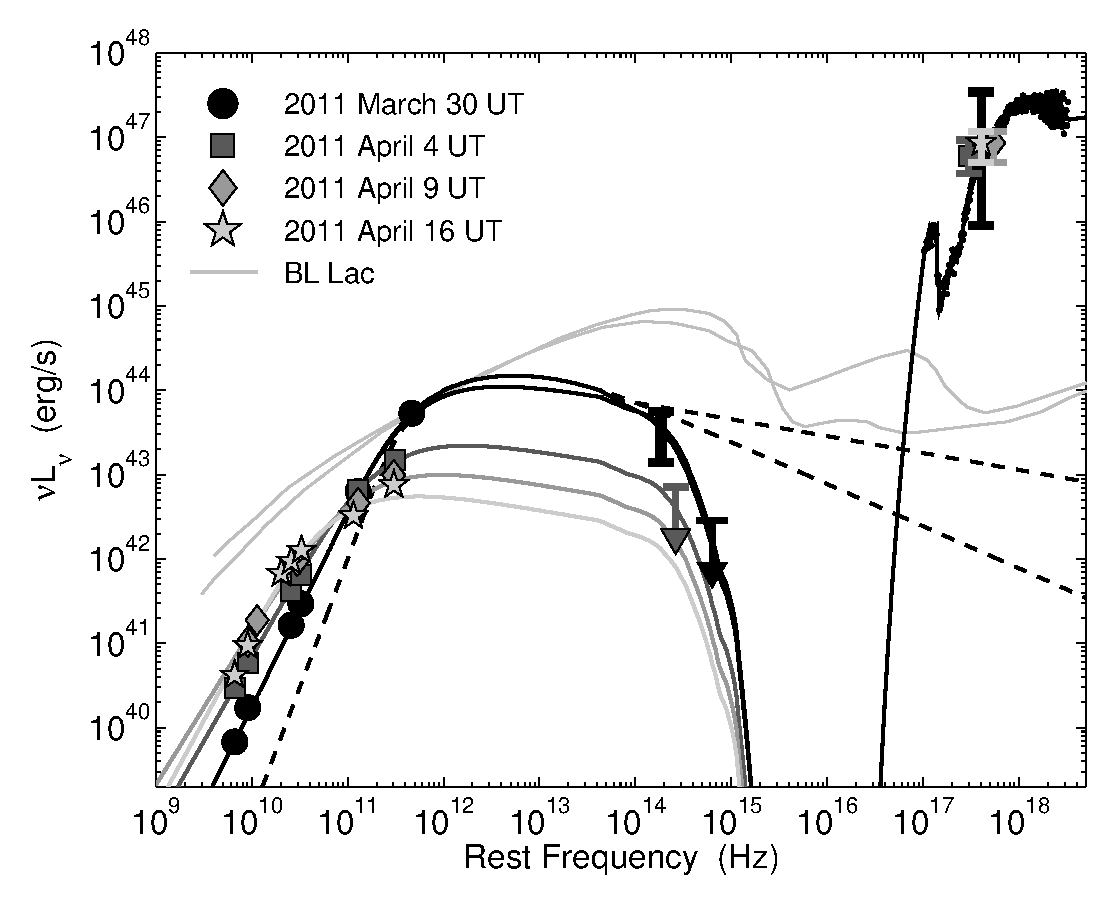
\psfig{file=figure2.eps,width=4.5in,angle=0}}
\caption[]{\small 
Spectral energy distributions (SEDs) of
Swift\,J164449.3+573451 from radio to X-rays point to synchrotron
emission from a relativistic outflow.  Our radio observations cover
decimeter to millimeter wavelengths at 5, 10, 15, and 22 d after the
initial $\gamma$-ray detection.  The NIR luminosity on March 30
can only be constrained within a factor of five due to the
unknown contribution from the host galaxy; on April 4 the NIR
upper limit is inferred from a {\it Hubble Space Telescope}
image\cite{ltc+11}.  Only an upper bound is available on the optical 
luminosity (black triangle) due to the lack\cite{ltc+11} of variable 
emission.  The flux in the soft X-ray band is highly variable on March
30, but is more quiescent at 10, 15, and 22 d (extrema marked by vertical 
bars and mean brightness by solid symbols with points at 10 and 15 d shifted slightly 
in frequency for clarity).  The radio, NIR, and optical data are well 
modeled by an evolving synchrotron spectrum (solid lines) with 
a large rest-frame optical extinction of $A_V\simgt 3$ mag.  The synchrotron 
curves for the March 30 SED are for two values of the synchrotron cooling frequency: $\nu_c\approx
2\times 10^{13}$ Hz (steeper optically thin slope) and $\nu_c\simgt
2\times 10^{18}$ Hz (shallower optically thin slope).  This 
model cannot explain the large X-ray luminosity, which remains
nearly constant while the radio spectrum is evolving strongly.  A
representative model for the X-ray spectrum (data=black dots;
model=black line) includes power-law ($F_\nu\propto\nu^{0.9}$) and
blackbody ($kT\approx 1$ keV) components with significant absorption
($N_H\approx 2\times 10^{22}$ cm$^{-2}$), in agreement with the
large optical extinction.  Shown for comparison is the SED of the
canonical blazar BL Lac in two separate states (varying in peak
frequency and flux of the synchrotron component), normalized to the
luminosity of Swift\,J164449.3+573451 at 345 GHz.  The blazar SED
provides a poor match.
}
\label{fig:sed} 
\end{figure}


\clearpage 
\begin{figure}
\centerline{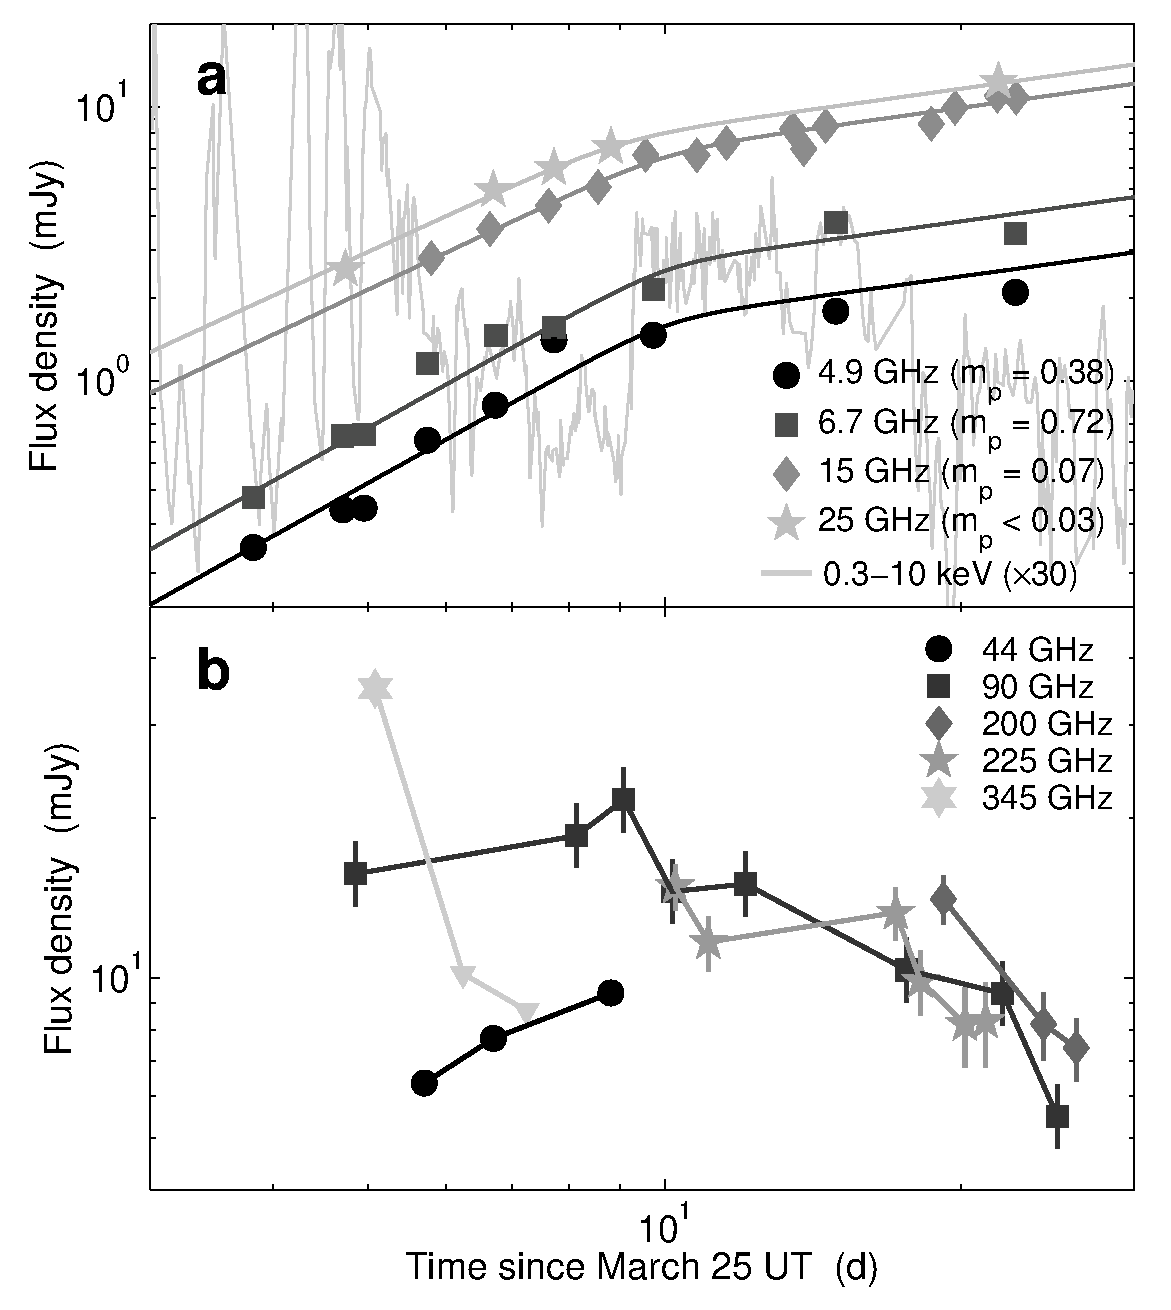
\psfig{file=figure3.eps,width=3.5in,angle=0}}
\caption[]{\small 
 Radio light curves of Swift\,J164449.3+573451 at
$5-345$ GHz reveal interstellar scintillation.  (a) Light curves at
$5-25$ GHz (error bars are smaller than symbols; see SI).  These data 
are from the EVLA, the AMI Large Array, and the OVRO
40-m telescope. The lines are broken power law fits to the $5-25$ GHz
light curves, using March 25 as the initial time.  The low
frequency light curves exhibit significant interstellar scintillation,
with the strongest modulation at 6.7 GHz.  To calculate the expected
interstellar scintillation we use the NE2001 Galactic Free Electron
Density Model\cite{cl02}.  For the line of sight to Swift\,J164449.3+573451 
($l=86.7111$, $b=39.4415$) the scattering measure is $2.2\times 10^{-4}$ kpc
m$^{-20/3}$.  With a scattering screen distance of $\sim 1$ kpc the
transition from weak to strong scattering occurs\cite{gn06} at 
$\nu_0\approx 10$ GHz, while the Fresnel scale is
$\theta_{F,0}\approx 1$ $\mu$as (sizes are given as radii).  At
frequencies above $\nu_0$ the modulation index is given by $m_p\propto
(\nu/\nu_0)^{-17/12}\,(\theta_s/\theta_{F,0})^{-7/6}$.  For
frequencies below $\nu_0$ refractive scintillation leads to
$m_p\propto (\nu/\nu_0)^{17/30}\,(\theta_s/\theta_r)^{-7/6}$, where
the refractive scale is $\theta_r=\theta_{F,0}(\nu/\nu_0)^{-11/5}$.
Comparing these results to the observed modulation we infer a size of
$\theta_s\approx 5$ $\mu$as.  Also shown is the {\it Swift} X-ray
light curve\cite{burrows11} binned on a timescale of 15 min and
multiplied by a factor of $1.3\times 10^{10}$ to fit on the same flux
density scale as the radio data.  The strong X-ray variability during
the first 10 d is not accompanied by similar order of magnitude
fluctuations in the radio bands, pointing to a distinct origin for the
radio and X-ray emission.  (b) Light curves at $44-345$ GHz from the
EVLA, CARMA, and the SMA (error bars are one standard deviation).
These frequencies are mainly in the decline phase and therefore
provide information on the peak of the synchrotron spectrum
(Figure~\ref{fig:sed}).  Upper limits at 345 GHz are marked by
triangles.
}
\label{fig:lc} 
\end{figure}

\end{document}
